\label{sec:NN}
Fully connected or feed-forward neural networks (NN) have a long history in high energy physics. The earliest usage of neural networks in particle physics were as part of the program of top physics measurements at the Tevatron\cite{Abazov:2006gd, Aaltonen:2008sy}. The fundamental element of a feed-forward neural network is called a layer. Multiple layers are stacked together connecting input variables to a predicted outcome which is evaluated against a known target value. A fully-connected network can have multiple internal (or hidden) layers between the input and output layers, and each hidden layer is composed of a series of trainable activation functions and weights that allow the network to identify and iteratively combine important features of the input space. A vector of relevant physics-level information (e.g. mass of two highest \pt jets, angle between measured objects, etc.) is constructed for each event and these vectors are then `fed forward´ through multiple layers in order to predict whether the event comes from a signal di-Higgs process or a background QCD process. A function (called the loss function) is chosen to quantify the difference between the model prediction and target values. The loss calculated after a single training iteration is used to adjust the internal network weights in the next training iteration through a process called backpropagation. The model is fully trained once the improvement in the loss between iterations falls beneath some user-defined threshold.

The NN trained for di-Higgs detection was built using the Keras~\cite{chollet2015keras} and Tensorflow~\cite{tensorflow} packages. The top twenty-two most separable reconstructed and event-level variables were used as the input variables for the NN. The complete network structure consists of the input layer, two hidden layers, and a single-node output layer. The first hidden layer contains 175 nodes with an L2 kernel regularizer ($\lambda$ = $10^{-4}$). The second hidden layer contains 90 nodes with no kernel regularizer. A batch normalization layer and a dropout (0.2) function are placed in between the two hidden layers to prevent over-fitting. Both hidden layers use a rectified linear (ReLU) activation function, while the output layer uses a sigmoid activation function. Several models were trained by individually tuning each hyperparameter over a reasonable range in order to produce a final optimized model. A schematic flowchart of the network structure is shown in Figure~\ref{fig:nn}.
%The sequential model was compiled using the ‘adam’ optimizer along with the ‘binary\_crossentropy’ loss method. Finally, the model was fit on the training data along with the validation data for 100 epochs. 

\begin{figure}[!h] 
\begin{center}
\includegraphics*[width=0.75\textwidth] {ffNN/figures/flowchart_ffNN.png}
\caption{Structure of the feed-forward neural network. The input variables are fed through two fully connected dense layers to classify events. One dropout layer and one batch normalization layer help mitigate over-fitting during training.}
  \label{fig:nn}
\end{center}
\end{figure}

The NN was trained for 25 epochs before the minimal loss-improvement threshold was met, and the results are shown in Figure~\ref{fig:results_nn}. The trained model obtained a maximum $S/\sqrt{B}$ = 2.40$\pm$0.08 when considering events with a signal prediction score > 0.94. This phase-space has a signal yield of 1659.9 events and a background yield of 477215.3 events.

\begin{figure}[!h] 
\begin{center}
   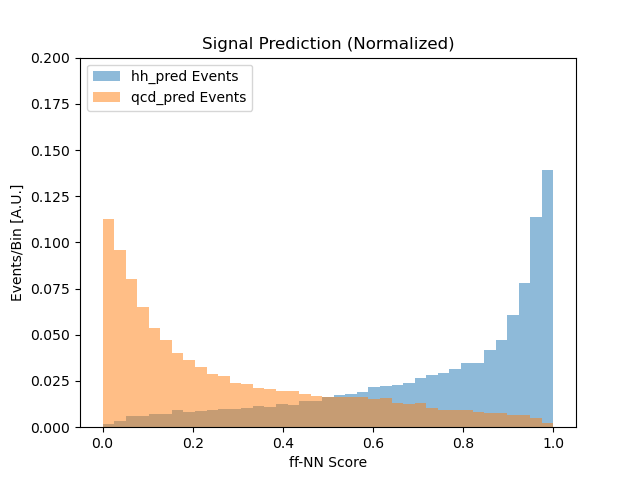
\includegraphics[width = 3in]{ffNN/figures/score_ffnn_v3}\\
\caption{Final predictions of the feed-forward network for signal and background samples.}
  \label{fig:results_nn}
\end{center}
\end{figure}

